\section{Theory}\label{sec:Theory}

\subsection{The System}
\subsubsection{The Potentials}

The Hamiltonian under investigation describes \(N\) bosons in a potential trap
of the form

\begin{equation*}
H = \sum_{i=1}^{N}\left( \frac{-\hbar^{2}}{2m}\nabla^{2}_{i} + V_{\text{ext}}(\vb{r}_{i})\right) + \sum_{i<j}^{N}V_{\text{int}}(\vb{r}_{i}, \vb{r}_{j})
\end{equation*}

where \(V_{\text{ext}}\) is the external potential of the trap and 
\(V_{\text{int}}\) is the internal potential between the particles. 
The external potential has an elliptical form, being anisotropic in the \(z\)-direction:

\begin{equation}
\label{eq:2}
V_{\text{ext}}(\vb{r}) = \frac{1}{2}m\left( \omega\left[ x^{2} + y^{2} \right] + \omega_{z}z^{2} \right).
\end{equation}

The internal potential is a hard shell potential, with infinite values when two bosons overlap:

\begin{equation*}
V_{\text{int}} = \begin{cases}
\infty, &\text{for } |r_{i} - r_{j}| \le 0\\
0, &\text{otherwise.}
\end{cases}
\end{equation*}

\subsubsection{Non-interacting Case}
For non-interacting bosons in a spherical with \(\beta = 1\) and \(a = 0\) the
system reduces to spherical harmonic oscillators where analytical solutions are
available. The trial wavefunction reduces to simply the product of one body
elements

\newcommand{\psit}{\Psi_T(\vb{r})}
\newcommand{\onebody}{\prod_{i}^{N}\exp{-\alpha\left[\left( x_i^2 + y_i^2 + \beta
		z_i^2\right)\right]}}
\begin{align*}
\psit = \prod_{i}^{N}\exp[-\alpha\left( x_{i}^{2}+y_{i}^{2}+z_{i}^{2} \right)] = \prod_{i}^{N}\exp(-\alpha \abs{r_{i}}^{2})
\end{align*}

while the Hamiltonian reduces to

\begin{align*}
H = \sum_{i}^{N} \frac{-\hbar^{2}}{2m}\nabla_{i}^{2} + \frac{1}{2}m\omega^{2}r_{i}^{2}
\end{align*}

which in natural units is

\newcommand{\lapl}[1]{\nabla_{#1}^2}
\begin{align*}
H = \frac{1}{2}\sum_{i}^{N} -\frac{1}{m}\lapl{i} + m\omega^{2}r_{i}^{2}.
\end{align*}

Applying the Hamiltonian gives the local energy as

\begin{align*}
E_{L} = \frac{\alpha d}{m} N + \left( \frac{1}{2}m\omega^{2} - \frac{2\alpha^{2}}{m} \right)\sum_{i}^{N}r_{i}^{2}
\end{align*}
where \(d\) is the dimension. As the factor \(\sum r_{i}^{2}\) is always
positive, its term should be minimized, which is accomplished by setting
\(\alpha = \frac{m\omega}{2}\), giving a minimal local energy of

\begin{equation}
E_{L} = \frac{\omega d N}{2}.
\label{eq:noninteracting}
\end{equation}

\subsubsection{Interacting Case}
The local energy for the full interacting case is much more complicated. The expression
evaluates to

\begin{align*}
E_{L} &= -\frac{1}{2m}\sum_{i}\bigg[4\alpha^{2}\left(  x_{k}^{2}\uvec{i} + y_{k}^{2}\uvec{j} + \beta^{2} z_{k}^{2}\uvec{k}  \right)\\
&-2\alpha(d-1+\beta)\\
&- 4\alpha\left(  x_{k}\uvec{i} + y_{k}\uvec{j} + \beta z_{k}\uvec{k}  \right)
\sum_{l\neq k} \frac{\vb{r}_{k}-\vb{r}_{l}}{r_{kl}}u^{\prime}\left( r_{kl} \right)\\
&+ \sum_{i\neq k}\sum_{j\neq k}\frac{\left( \vb{r}_{k}-\vb{r}_{i} \right)\left( \vb{r}_{k} -\vb{r}_{j} \right)}{r_{ki}r_{kj}}u^{\prime}\left( r_{ki} \right)u^{\prime}\left( r_{kj} \right)\\
&+ \sum_{l\neq k} \left( u^{\prime\prime}\left( r_{kl} \right)  + \frac{2}{r_{kl}}u^{\prime}(r_{kl})\right)\bigg]\\
&+ \sum_{i}V_{\text{ext}}(\vb{r}_{i}) + \sum_{i<j}V_{\text{int}}\left( \vb{r}_{i}, \vb{r}_{i} \right).
\end{align*}

\subsection{Variational Monte Carlo}
In order to find a good candidate wavefunction for a given potential, one can
employ the \textit{variational principle}. One starts by guessing a trial
wavefunction \(\ket{\Psi_{T}}\) and estimating the trial energy, which is
guaranteed to be equal to or higher than the true ground state energy \(E_{0}\):
\begin{equation}
  \label{eq:1}
  E_{0} \le E = \frac{\ev{H}{\Psi_{T}}}{\ip{\Psi_{T}}}.
\end{equation}

If \(\ket{\Psi_{T}}\) is an eigenfunction of the Hamiltonian, the variance
\(\sigma^{2}\) will be minimal

\begin{equation*}
  \sigma^{2} = \frac{\ev{H^{2}}{\Psi_{T}}}{\ip{\Psi_{T}}} -\left( \frac{\ev{H}{\Psi_{T}}}{\ip{\Psi_{T}}} \right)^{2} = 0.
\end{equation*}

The variational principle expands on this idea by letting \(\ket{\Psi_{T}}\) be
a functional class of a \textit{variational parameter} \(\alpha\). By varying
\(\alpha\) one can find the optimal trial wavefunction within the functional
class by minimizing \(\sigma^{2}\). 

Only a small collection of potentials have analytical solution using the
variational principle. For most potentials, one must numerically
integrate~\eqref{eq:1} using Monte Carlo integration.

For a stochastic variable \(x\) with probability density function \(p(x)\), the
average \(\left< x \right>\) is defined as
\begin{equation*}
  \left< x \right> = \int_{\mathbb{R}} xp(x)\dd x.
\end{equation*}
By sampling the stochastic variable \(M\) times, the average can be approximated
by 

\begin{equation*}
  \expval{x} = \int_{\mathbb{R}} xp(x)\dd x \approx \frac{1}{M}\sum_{i=1}^{M}x_{i}p(x_{i}).
\end{equation*}

Applying this to an observable \(\mathcal{O}\), we have

\begin{align*}
  \expval{\mathcal{O}} &= \ev{\mathcal{O}}{\Psi}\\
                       &= \int \dd \vb{r} \Psi^{*}\mathcal{O}\Psi \\
                       &= \int \dd \vb{r} \abs{\Psi}^{2} \frac{1}{\Psi}\mathcal{O}\Psi\\
  &= \frac{1}{M} \sum_{i=1}^{M}p(\vb{r})\mathcal{O}_{L}.
\end{align*}

where \(\abs{\Psi}^{2}\) is defined as the probability density function, and
\(\frac{1}{\Psi}\mathcal{O}\Psi\) the \textit{local operator}.

The local trial energy can then be defined as
\begin{equation*}
  E_{L} =\frac{1}{\Psi_{T}}H\Psi_{T}
\end{equation*}
which can be computed using Monte Carlo integration as

\begin{align*}
  \expval{E_{L}} \approx \frac{1}{M}\sum_{i=1}^{M} p(\vb{r}_{i})E_{L}(\vb{r}_{i}).
\end{align*}

The goal is therefore to minimize minimizing \(\sigma^{2} = \expval{E_{L}^{2}} -
\expval{E_{L}}^{2}\) over the variational parameter \(\alpha\).


\subsection{Onebody Density}

A useful way to understand a many body system is to integrate over all
dimensions except for one, yielding the \textit{one body density}
\(\rho(\vb{r})\), defined as

\begin{align*}
  \rho( \vb{r} ) = \int \dd \mathbf{r}_{2} \ldots \dd \mathbf{r}_{N} \left| \psit \right|^{2}.
\end{align*}

It is a scaled probability density function giving the number of particles
within the volume \(\Delta \vb{r}\) as \(\rho(\vb{r})\Delta \vb{r}\).
By convention the integral over all \(\dd \vb{r}\) yields the total number of
particles in the system, \(N\).


\subsection{Metropolis-Hastings}

The estimate of the local energy relies on samples from the trial wave function.
To get a physical value, the configuration of the particles must be as physical
and probable. As the configuration achieving this is unknown, the configuration
space must be explore. This is done through Monte Carlo simulation, more
specifically by using the Metropolis-Hastings algorithm.

At each MC step a single particle is chosen at random, and a change to its
position is proposed by moving it a fixed step length \(\Delta\) and computing the
ratio between new and old probability densities
\begin{align*}
\omega = \frac{P\left( \vb{r}_{r}, \ldots, \vb{r}_{k}^{*}, \ldots, \vb{r}_{n} \right)}{P\left( \vb{r}_{r}, \ldots, \vb{r}_{k}, \ldots, \vb{r}_{n} \right)}
=  \frac{\left| \Psi_{T}\left( \vb{r}_{r}, \ldots, \vb{r}_{k}^{*}, \ldots, \vb{r}_{n} \right)\right|^{2}}{\left| \Psi_{T}\left( \vb{r}_{r}, \ldots, \vb{r}_{k}, \ldots, \vb{r}_{n} \right)\right|^{2}}
\end{align*}
where \(\vb{r}^{*}\) denotes a modified position.
If the ratio \(\omega\) is greater
than a
uniformly distributed number \(\theta \in [0, 1]\), the move is accepted.
This ratio can often be reduced analytically to obviate the need for recomputing
the entire probability density each step.



\subsection{Neural Networks}

\begin{figure}[t]
  \label{fig:neuralnet}
  \centering
  \def\layersep{2.5cm}
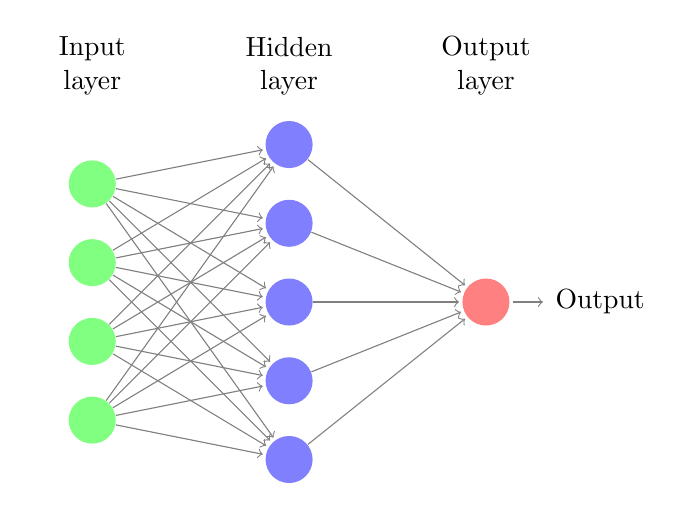
\begin{tikzpicture}[shorten >=1pt,->,draw=black!50, node distance=\layersep]
    \tikzstyle{every pin edge}=[<-,shorten <=1pt]
    \tikzstyle{neuron}=[circle,fill=black!25,minimum size=17pt,inner sep=0pt]
    \tikzstyle{input neuron}=[neuron, fill=green!50];
    \tikzstyle{output neuron}=[neuron, fill=red!50];
    \tikzstyle{hidden neuron}=[neuron, fill=blue!50];
    \tikzstyle{annot} = [text width=4em, text centered]

    % Draw the input layer nodes
    \foreach \name / \y in {1,...,4}
    % This is the same as writing \foreach \name / \y in {1/1,2/2,3/3,4/4}
        \node[input neuron] (I-\name) at (0,-\y) {};

    % Draw the hidden layer nodes
    \foreach \name / \y in {1,...,5}
        \path[yshift=0.5cm]
            node[hidden neuron] (H-\name) at (\layersep,-\y cm) {};

    % Draw the output layer node
    \node[output neuron,pin={[pin edge={->}]right:Output}, right of=H-3] (O) {};

    % Connect every node in the input layer with every node in the
    % hidden layer.
    \foreach \source in {1,...,4}
        \foreach \dest in {1,...,5}
            \path (I-\source) edge (H-\dest);

    % Connect every node in the hidden layer with the output layer
    \foreach \source in {1,...,5}
        \path (H-\source) edge (O);

    % Annotate the layers
    \node[annot,above of=H-1, node distance=1cm] (hl) {Hidden layer};
    \node[annot,left of=hl] {Input layer};
    \node[annot,right of=hl] {Output layer};
\end{tikzpicture}
  \caption{Diagram of an artificial neural network with one fully connected hidden layer. Taken
    from \url{http://www.texample.net/tikz/examples/neural-network/}}
\end{figure}


Neural networks is a machine learning algorithm inspired by biological neurons,
and has achieved impressive performance on a wide class of problems. A neuron is
modeled by a \textit{perceptron}, with perceptrons stacked together in layers
and layers stacked together into a network architecture. The first layer takes
an input vector \(\vb{x}\) of \(d\) features and produces an \textit{activation}
\(a_{i}(\vb{x})\). The activation is feed into the next layer, called
\textit{hidden layer}, and so on until
the last layer, the \textit{output layer}.

A layer transforms its input but first applying an
affine transformation on the form

\begin{align*}
  z^{(i)} = W^{(i)}\vb{x} + b^{i}
\end{align*}

with \(W^{i}\) being the \textit{weights} of layer \(i\) and \(b^{i}\) its
\textit{bias}. This is followed by a non-linear transformation

\begin{align*}
  a_{i}(\vb{x}) = f_{i}(z^{(i)})
\end{align*}
The \textit{activation function } \(f_{i}\) is specific to each layer. 
The activation function of the output layer determines whether the network is a
classifier, in which the function is a sigmoid or softmax function, or regression,
where the function are unbounded linear functions.

The combination of linear and non-linear transformations allows a network to
approximate any function to arbitrary precision, a result known as the universal
approximation theorem\cite{mehta}. In order to achieve this expressive power,
the network has to be trained. This is done by an algorithm known as
\textit{backpropagation}.

\subsubsection{Backpropagation}

To train a network, a cost function is optimized, often being the mean square error.  The optimization is done by gradient descent, where an input is fed
forward through the network, compared to the expected output, and the error is
fed backwards and used to update the weights and biases. This backpropagation of
the error is essentially the chain rule from calculus applied recursively.

The four equations of backpropagation are

\begin{align*}
  \delta_{j}^{l} &= \pdv{E}{a_{j}^{l}}f\prime\left( z_{j}^{l} \right)\\
  \delta_{j}^{l} &= \pdv{E}{b_{j}^{l}}\\
  \delta_{j}^{l} &= \left( \sum_{k}\delta_{k}^{l+1}w_{kj}^{l+1} \right)f\prime\left( z_{j}^{l} \right)\\
  \pdv{E}{w_{jk}^{l}} &= \delta_{j}^{l}a_{k}^{l-1}
\end{align*}

A deeper explanation of these equation and their derivation can be found in
literature, such as~\cite{mehta}.

\subsection{Recurrent Neural Networks}

\begin{figure}[ht]
  \centering
  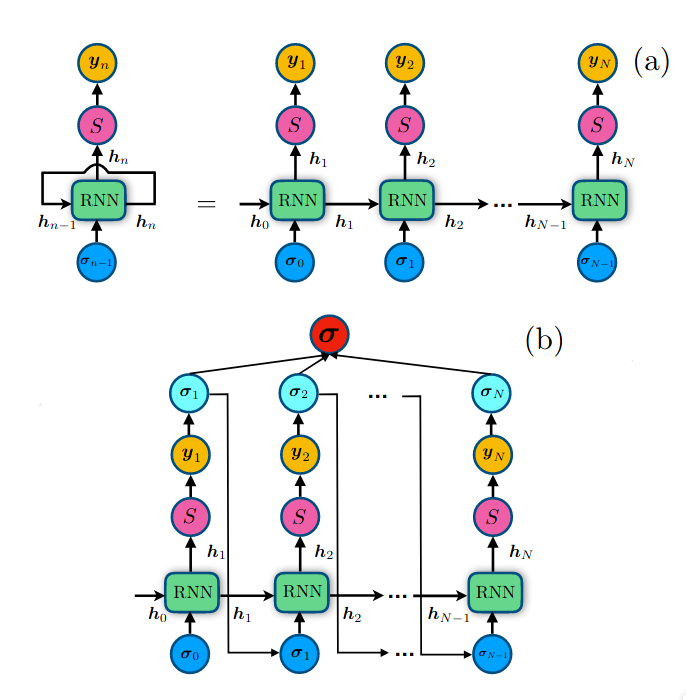
\includegraphics[width=\columnwidth]{figures/rnn.png}
  \caption{\label{fig:rnn} Illustrations of common recurrent neural net. (a)
    Left: A RNN cell takes a sequence of inputs \(\left\{  \mathbf{\sigma}\right\}\) that are
    combined with the hidden state \(\vb{h}_{n-1}\) to produce an updated hidden
    state \(\vb{h}_{n}\), encoding information about \(\mathbf{\sigma}_{n-1}\).
    The hidden state is here propagated through a softmax function \(S\) to
    produce the output \(\vb{y}_{n}\), but note that a softmax is not required.
    Right: The unrolled version, more clearly showing the sequential nature of
    RNN. (b) A representation of autoregressive sampling of RNNs. Instead of
    taking external sequential input, the RNN itself generates the sequence
    \(\left\{ \mathbf{\sigma} \right\}\) from an initial state
    \(\mathbf{\sigma}_{0}\). The output of each propagation through the RNN is
    fed back into the network, with their combination being the ultimate output.
    Edited
    version of figure from~\cite{hibatallah2020recurrent}.}
\end{figure}

A recurrent neural network (RNN) is an extension to vanilla neural networks. Its purpose is to
capture the current context through a hidden state whereby long
range correlations can be modeled. Its usefulness is apparent when there are
strong correlations between sequential inputs, such as time varying signals.

A RNN can model a correlated probability distribution where a new sample is
entirely determined by previous samples. 
Letting \(\bm{\sigma} = \left(\sigma_{1}, \sigma_{2}, \ldots,
  \sigma_{N}\right)\)  denote a configuration of \(N\) samples, the
probability of observing a specific configuration is
\begin{equation*}
  P(\bm\sigma) = P(\sigma_{1})P(\sigma_{2}|\sigma_{1})\cdots P(\sigma_{N}|\sigma_{N-1},\ldots,\sigma_{1})
\end{equation*}
%Constructing a RNN allows for an efficient sampling of \(P(\sigma)\) without
%endowing any structure on the distribution.

This is achieved through the use of a \textit{recurrent cell}. The basic
structure of a recurrent cell is and update of the hidden state by 
combining it with the input, and using the updated state to compute the output.
The hidden state \(\vb{h}_{n-1}\)
contains information about the previous forward pass, and is updated by
concatenating the hidden state to an input state \(\bm{\sigma}_{n-1}\) and passing
it through a non-linear activation function \(f\) such that

\begin{equation*}
  \vb{h}_{n} = f(W\left[ \vb{h}_{n-1};\bm{\sigma}_{n-1} \right] + \vb{b})
\end{equation*}
with \(\vb{h}_{n-1},\vb{b}\in \mathbb{R}^{d_{h}}\),
\(\bm{\sigma}_{n-1}\in\mathbb{R}^{d_{v}}\) and \(W\in\mathbb{R}^{d_{h}\times
  (d_{h}+d_{v})}\) where \(d_{h,v}\) are the dimensions. The activation function
is often \(\tanh\) due to its desirable properties.

The updated hidden state is propagated forward through a softmax layer \(S\) to yield
the coefficient of each \(\sigma_{n}\):
\begin{equation*}
  \vb{y}_{n} = S(U\vb{h}_{n} + \vb{c})
\end{equation*}
where \(U\in\mathbb{R}^{d_{v}\times d_{h}}\) and
\(\vb{c}\in\mathbb{R}^{d_{v}}\).

The softmax function ensures that the
coefficients \(\vb{y}_{n}\) sum up to \(1\), forming a probability distribution
over the states \(\sigma_{n}\). This allows for the full probability to be
computed as
\begin{equation*}
  P(\bm{\sigma}) = \prod_{n=1}^{N}\vb{y}_{n}\cdot \sigma_{n}.
\end{equation*}

To sample \(N\) samples from the RNN probability distribution, one begins with
initial states \(\bm{\sigma}_{0}\) and \(\vb{h}_{0}\), computing the resulting
\(\sigma_{1}\), one-hot encoding it to obtain \(\sigma_{1}\), repeating the
computation with \(\sigma_{1}\) and the now updated \(\vb{h}_{1}\), and
iterating until \(N\) samples are obtained.

\subsection{RNN Wave functions}

In general, wave functions are complex valued. Our problem domain, however,
only concerns itself with stochastic many-body Hamiltonian at ground state
energy. These yield strictly real and positive wave
functions\cite{Sharir_2020}. For a many-body system of \(N\) particles, the
total wave function in position basis can be written as the product of all conditional single particle wave
functions

\begin{equation*}
  \Psi(\vb{x}_{0}, \vb{x_{1}}, \ldots, \vb{x}_{N}) = \prod_{i=0}^{N}\psi_{i}(\vb{x}_{i}|\vb{x}_{i-1}, \ldots, \vb{x}_{0})
\end{equation*}
for positions \(\left\{  \vb{x}_{i}\right\}\). That each \(\psi_{i}\) is normalized is a
sufficient condition for the total wave function to be
normalized\cite{Sharir_2020}. However, this was not done here, as the wave
function itself is only used as a ratio in the Metropolis sampling, eliminating 
the need for normalizing.

%%% Local Variables:
%%% mode: latex
%%% TeX-master: "../main"
%%% End:
